
\chapter{Introduction}
  Vulnerabilities in software can have serious consequences, including reputation damage,
  financial losses, or even loss of life in the case of critical infrastructure systems. Most of them
  are introduced during the development process as a result of hidden errors, which might not appear
  suspicious at first. The system and its users or their data are at~risk until flaws are patched.
  That is the main reason and motivation why it is important to~constantly improve the security of products.

  Cloned vulnerabilities are security weaknesses that are introduced into a software system
  when code is copied or reused from another system that contains the vulnerability.
  These vulnerabilities can be difficult to detect and fix, because they are not necessarily introduced
  intentionally, instead, they are inherited from the source code that was copied or reused. In software
  engineering, the approach of cloning similar functional parts already implemented in~other applications
  is usually applied. It makes the development of new products or adding features to existing ones swifter.

  For this case, cryptocurrencies are a good example which became very popular in recent years.
  Namely, Bitcoin, an Open-Source peer-to-peer electronic cash system created by Satoshi Nakamoto~\cite{bitcoin}
  inspired many new projects that joined the cryptocurrency market. Lots~of them were created
  as derivatives of Bitcoin with the idea to extend or improve its features. Cloning helped to speed up
  the development of new coins by inheriting its base infrastructure.

  Although, neither a large-scale project developed by the community as Bitcoin is always perfect. Plenty of
  vulnerabilities were discovered in its code base which were accordingly documented and are stored
  and tracked in vulnerability databases. As there are many other coins that share its code, it is possible
  that they also share the same vulnerabilities. The question inspired this work to develop a monitoring tool
  with the goal to analyze the~threat and help with the detection of vulnerable code and its occurrence in
  cloned projects, as the identification is not an easy but rather costly and exhaustive process
  and after identification yet also patching the issue is desired.

  The prevalence of code reuse and the increasing complexity of software systems makes cloned vulnerabilities
  an important issue to consider in software development and maintenance. This thesis aims to study the
  characteristics and impacts of cloned vulnerabilities and to identify effective approaches for detecting
  and mitigating them. The proposed tool in this work considers disclosed vulnerabilities which means
  that the issue was already patched in the project that was originally affected by it. Thanks to this fact
  the tool can identify an~issue, the affected code in the original project, and candidate projects with
  the~probability of vulnerability inheritance. Additionally, the tool can also propose a patch for
  the detected threat.

  An existing tool, with the same goal described above, was implemented in a project named CoinWatch~\cite{CoinWatch}
  with an aim on vulnerabilities in cryptocurrencies. The CoinWatch inspired this work
  with an idea to bring improvements, extensions, and a graphical user interface for wider and simplified
  usage of the tool for detecting and mitigating cloned vulnerabilities.

  This thesis begins with a basic introduction to the problem and the motivation for why it is relevant
  to deal with. Chapter \ref{chapter:vulnerabilities} explains and takes a closer look at vulnerabilities
  and the basic terminology connected with them. In Chapter \ref{chapter:clonedVulnerabilities}, clones of source
  code, current detection tools and approaches are described and analyzed. Afterwards, Chapter \ref{chapter:design}
  describes a draft of the tool built for detecting cloned vulnerabilities. The next two Chapters
  \ref{chapter:implementation} and~\ref{chapter:experimentation} contain implementation details
  and an evaluation of the developed product. The final Chapter \ref{chapter:conclusion} concludes this work
  with potential improvements for future work.


\chapter{Vulnerabilities in Software Applications}
\label{chapter:vulnerabilities}
  Software vulnerabilities and exposures are weaknesses or flaws in software products that are
  exploitable in a cyber attack. The exploitation of a vulnerability can allow an attacker unauthorized
  access, elevation of privileges or denial of service~\cite{SoftwareVulnerabilities}.
  Most of the known vulnerabilities are associated with dealing with input provided by a user
  of the application. For instance, some frequent types of vulnerabilities include buffer overflows,
  cross site scripting, and SQL injections~\cite{vulnerabilities}. The mistakes causing these issues
  can be introduced during the development process or by using insecure libraries and frameworks.

  This Chapter will present an example of a cyberattack and its consequences that was performed a few years ago
  to introduce the severity of this topic. Accordingly, also some general ways to improve the security of applications
  will be presented. This is followed by a~description of identifiers related to evaluating vulnerabilities
  and public databases storing details about them.

  \section{Real-world Example of Exploitation}
  The consequences of vulnerabilities in software applications can be quite serious like data breaches,
  theft of sensitive information, or damage to a product infrastructure. For instance, consider
  vulnerability, in Microsoft Windows implementation of Server Message Block protocol, with an identifier
  CVE-2017-0144. An exploitation of this flaw, by sending crafted packets, allows remote attackers to run
  arbitrary code on a target machine. This defect facilitated the spreading of worm-like ransomware
  \emph{WannaCry} through the network in~2017, which affected many organizations, companies,
  and individuals~\cite{WannaCry}. Figure~\ref{wannacryDistribution} depicts the spread of \emph{WannaCry} ransomware.
  % https://nvd.nist.gov/vuln/detail/CVE-2017-0144
  % https://www.zdnet.com/article/ransomware-an-executive-guide-to-one-of-the-biggest-menaces-on-the-web/

  Ransomware is a type of malicious software, that locks up the victim's data or device and threatens to delete
  or keep it locked unless a ransom is paid to an attacker~\cite{Malware}. In the case of \emph{WannaCry},
  the malware would encrypt files on the victim's device and ask for a ransom of value 300 USD in Bitcoin
  if paid within the first three days, otherwise, the value would be doubled for the next four days and if
  not paid at all, the files would be lost forever.
  % https://www.ibm.com/topics/ransomware
  % https://www.csoonline.com/article/3227906/wannacry-explained-a-perfect-ransomware-storm.html

  In order to mitigate repeated occurrences and time consuming process of patching, each
  vulnerability and exposure is documented and stored in a database, so repeated mistakes in implementation
  can be mitigated or fixed faster. This source provides valuable information for the public,
  security engineers, and for tools working with weaknesses in software applications to improve
  cyber security.

  \begin{figure}[h]
    \centering
    \includegraphics[width=0.9\textwidth]{obrazky-figures/wannacry_distribution_bc.pdf}
    \caption{WannaCry ransomware distribution}
    \label{wannacryDistribution}
  \end{figure}

  \section{Prevention and Mitigation}
  Preventing and mitigating software vulnerabilities is crucial for ensuring the security and reliability
  of developed software. This section presents some secure coding practices for the prevention
  and mitigation of weaknesses from being introduced during the development of a~product.

  \subsection*{Input Validation and Sanitization}
    An input of an application or service can have different sources which can be divided based on trustworthiness.
    For example, internal communication between services might be considered a trusted source. On the other side,
    Input from a user is considered to be an untrusted source because the data received can be anything.
    This makes it important to validate it properly, so that malformed input will not harm the system or lead
    to unexpected behaviour. An~example of insufficient validation are SQL injections. To improve input
    validation these points should be considered:
    \begin{itemize}
      \item check all inputs from untrusted sources
      \item check usage of proper character sets (UTF-8, ASCII, ...)
      \item encode data to a common character set before validation
      \item validate all received data for type, length, format, and range
      \item validate received data against a "white" list of allowed characters, when possible
      \item process special and hazardous characters with increased precision to address double encoding or other
            forms of obfuscation attacks
      \item all validation failures should result in input rejection
    \end{itemize}

  \subsection*{Output Encoding and Sanitization}
    When it comes to a trusted source of messages between services, some checks might be omitted as internal
    communication can be performed through an internal interface. Omitting of some validations, in this case,
    can benefit in better performance of the system. To achieve this goal it is essential to comply with
    all items mentioned in the previous subsection, so the exchanged messages should be correctly encoded
    and sanitized. Sanitization should be mainly done on data for commands to the operating system and queries
    for SQL, XML, and LDAP.

  \subsection*{Authentication and Password Management}
    Authentication is a process of validating the identity of a user, device, or system. It is used for
    ensuring restricted access to private resources or certain actions. Some authentication methods
    are:
    \begin{itemize}
      \item passwords -- typically used in combination with a user name
      \item two\,-factor authentication (2FA) -- this method requires two different forms of authentication
            to validate identity
      \item biometric authentication -- this type requires physical or behavioural actions, like
            face recognition or fingerprint, for identification
    \end{itemize}
    By implementing strong authentication methods into the system, organizations can prevent identity theft
    and protect against unauthorized access. Here are some practices on implementation, configuration
    and password management improvement:
    \begin{itemize}
      \item require authentication for all resources, except for those intended to be public
      \item authorization should be fail secure
      \item credentials should be stored only as cryptographically strong one-way salted hashes of passwords
            and storage should be writeable only by the application
      \item validate authentication only on completion of all input fields, especially in case of sequential
            authentication
      \item use only HTTP POST request for sending authentication data
      \item enforce higher password complexity -- length, numeric and/or special characters
      \item enforce account disabling after a number of failed login attempts, the duration should
            be sufficient to discourage guessing credentials by brute-force attack, but not to allow
            denial-of-service attack
      \item notify the user on password change
      \item allow next password change at least after one day from the last change
    \end{itemize}

  \bigskip

  More advice on secure coding practices can be found in~\cite{SecureCodingPractices}. Nevertheless, mistakes
  tend to slip into production versions of software. At this stage, other options are to use vulnerability
  scanning tools, write automated tests or perform penetration testing to discover hidden weaknesses, before
  they are exploited. Scanning tools are a form of static analysis. They work by searching the application's
  code/binary for vulnerable patterns. Details of such tools are analysed in the next Chapter
  \ref{chapter:clonedVulnerabilities}. Automated tests and penetration testing are forms of dynamic analysis.
  They discover run-time issues in the built and running application or its parts.

%  \section{Types of Software Errors}
%  Vulnerabilities are often caused by a coding mistake during development. This section presents a variety
%  of types of errors, which are mostly the result of forgotten validations mentioned in the previous section.
%  It is also important to note that the probability of these errors occurring is affected by the programming
%  language used and its capabilities, such as memory management. Below are described examples of issues frequently
%  contained within CVEs.~\cite{UnforgivableVulnerabilities}
%  \subsection*{Buffer Overflow}
%  \subsection*{Cross Site Scripting}
%  \subsection*{SQL Injection}

  \section{Identifiers Related to Security Vulnerabilities}
  This Section introduces identifiers which are used to evaluate and address vulnerabilities and the most popular
  publicly available databases storing records about disclosed weaknesses.

  \subsection*{CPE -- Common Platform Enumeration}
    CPE refers to a standardized method for describing and identifying abstract classes of software
    and hardware products present in an organization's computing infrastructure. The standard was created
    by the National Institute of Standards and Technology (NIST) as~the part of the Common Vulnerabilities
    and Exposures (CVE) program. The current version of CPE is 2.3 and is used to identify products
    in vulnerability databases. It is represented as formatted string binding with colon-delimited
    list of components prefixed with the string "\texttt{cpe:2.3:}"~\cite{CPEnaming}.\\
      \centerline{\texttt{cpe:2.3: part : vendor : product : version : update : edition :}}\\
      \centerline{\texttt{language : sw\_edition : target\_sw : target\_hw : other}}

  \subsection*{CWE -- Common Weakness Enumeration}
    CWE is a community-developed formal list of common software and hardware weakness types that
    have security ramifications, which was released in 2006. The CWE database is maintained by the MITRE Corporation
    and as of 28th December 2022, it contains 933 records. The main goal of CWE is to stop vulnerabilities
    at the source by educating software and hardware architects, designers, programmers, and acquirers
    on how to eliminate the most common mistakes before products are delivered~\cite{CWE}.

    The severity of weaknesses can be evaluated by Common Weakness Scoring System (CWSS). It provides a method
    for prioritizing software weaknesses. It is a collaborative, community-based effort that is addressing
    the needs of its stakeholders~\cite{CWSS}.

    \noindent Current top three weaknesses are~\cite{CWEtop25}:
    \begin{itemize}
      \item \textbf{CWE-787} -- Out-of-bounds Write
      \item \textbf{CWE-79} -- Improper Neutralization of Input During Web Page Generation ('Cross-site Scripting')
      \item \textbf{CWE-89} -- Improper Neutralization of Special Elements used in an SQL Command ('SQL Injection')
    \end{itemize}

  \subsection*{CVSS -- Common Vulnerability Scoring System}
  CVSS captures technical characteristics of software, hardware and firmware vulnerabilities. It attempts
  to assign severity scores to vulnerabilities. The score is in the range of 0.0 -- 10.0, where higher numbers represent
  more severe vulnerabilities. The metric is composed of three metric groups -- base, temporal and environmental --
  and helps with the prioritization of vulnerabilities~\cite{CVSSFirst, CVSSresearchgate}.

  \begin{figure}[h]
    \centering
    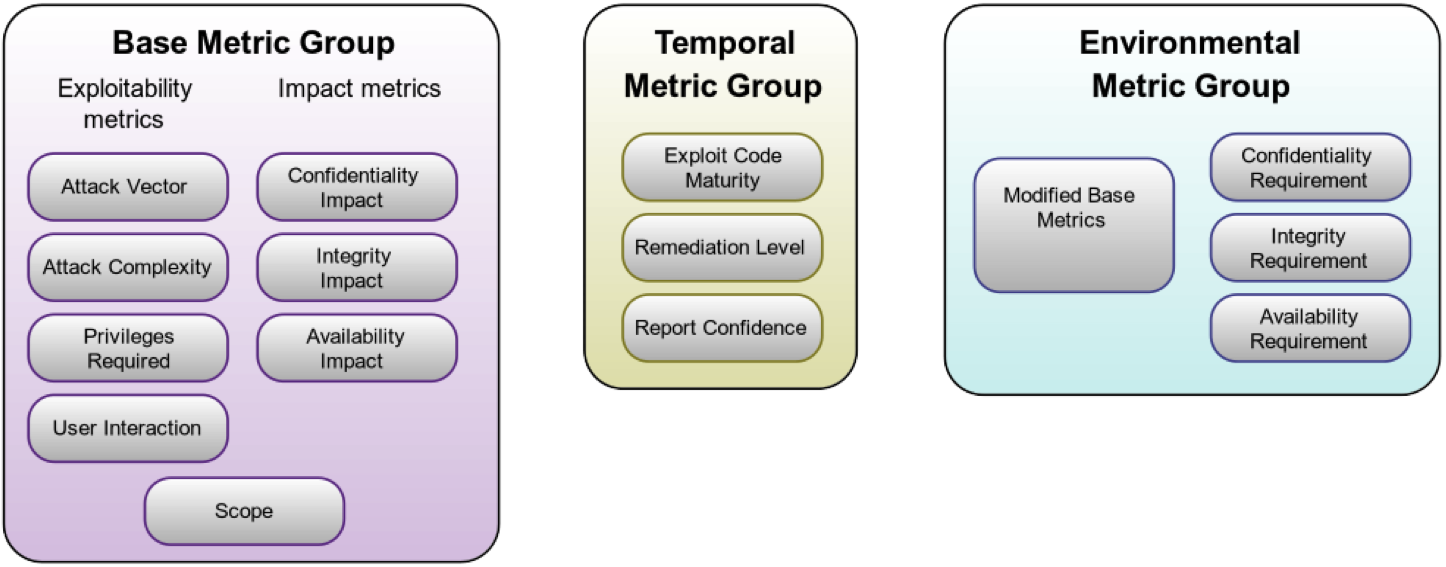
\includegraphics[width=0.9\textwidth]{obrazky-figures/cvss_metric_groups.png}
    \caption{Three CVSS metric groups. Source:~\cite{CVSSFirst}}
  \end{figure}

%   https://www.first.org/cvss/v3-1/cvss-v31-specification_r1.pdf
%   https://www.researchgate.net/publication/311694508_The_Common_Vulnerability_Scoring_System_CVSS_generations_-_usefulness_and_deficiencies

  \section{Vulnerability Databases}
  % https://wiww.researchgate.net/publication/316971384_Analyzing_Vulnerability_Databases
  In 1989 the Computer Emergency Response Team (CERT) was established at the Software Engineering Institute
  at Carnegie Mellon University to find, collect and publish all information about known vulnerabilities.
  After CERT displayed all collected vulnerabilities publicly, they started to appear in many new databases
  with different formats of weakness information. The most popular vulnerability databases were analysed
  in~\cite{VulnDBs}, but as of December 2022, some of them are shut down or not maintained.

  \subsection*{CVE -- Common Vulnerabilities and Exposures}
    CVE is a list of publicly disclosed computer security flaws. It was released in 1999, at a time when
    most cybersecurity tools used their own databases, names and evaluations of weaknesses. Now, CVE provides
    a database and a unified standard for naming information security vulnerabilities.

    The process of creating a new CVE identifier begins with discovering and reporting a potential security
    vulnerability. The information is accordingly assigned a unique CVE identifier by a CVE Naming Authority
    (CNA) and posted to the list on the CVE website by an editor. The MITRE Corporation functions as the editor
    and primary CNA~\cite{CVE}.

    Each entry in the list contains the following fields: CVE identifier number, brief description and references.
    The CVE identifier number format looks like "\texttt{CVE-YYYY-NNNN}", where
    '\texttt{Y}' refers to a year of creation and '\texttt{N}' is unique number assigned to the vulnerability.
    As~of 29th December 2022, the database contains 191\,855 CVE records\footnote{\href{https://cve.mitre.org}
    {https://cve.mitre.org}} and is synchronized with the following database.

  \subsection*{NVD -- National Vulnerability Database}
  The NVD was established in 2005 to provide the U. S. government with a repository of data about software
  vulnerabilities. It is a product of the National Institute of Standards and Technology (NIST) to provide
  vulnerability management information. The NVD can be used to prioritize the vulnerabilities to address
  in order to secure important systems.

  The database is based on and synchronized with the CVE list and enhances the base CVE scheme for vulnerability
  severity metrics and updates them when new information about the vulnerability is provided. CVSS is used
  for evaluation and helps to understand the potential severity of each vulnerability. NIST works directly
  with vendors and researchers to assure the quality of published data and provide the public with accurate
  scoring data~\cite{NVD}.

  Information about vulnerabilities is accessible to the public via the web page or REST API provided
  by the organization. As~of 29th December 2022, the database contains 203\,312 records providing the following
  data\footnote{\href{https://nvd.nist.gov/general/nvd-dashboard}{https://nvd.nist.gov/general/nvd-dashboard}}:
  \begin{itemize}
      \item Base CVE Entry Schema -- Identification, Description, References
      \item Source Identifier -- Reporter
      \item Publication Time
      \item Last Modification Time
      \item Status
      \item Metrics -- CVSS
      \item Weaknesses -- contained CWEs
      \item Configurations -- CPE
  \end{itemize}

%  \subsection*{VulnDB}
%  The VulnDB contains comprehensive vulnerability intelligence and provides actionable information about
%  the latest security vulnerabilities. The contents of the database are available via their web portal
%  or RESTful API. It allows organizations to search and be alerted on the latest vulnerabilities
%  in end-user software, libraries and dependencies. This database states to contain 307,250 vulnerabilities
%  and is a part of a threat intelligence platform provided by a company named Flashpoint which acquired Risk
%  Based Security (RBS). RBS is original founder of the VulnDB, previously named Open Sourced Vulnerability
%  Database (OSVDB).

\newpage


\chapter{Cloned Vulnerabilities}
\label{chapter:clonedVulnerabilities}
Cloned vulnerabilities are weaknesses propagated by reusing source code. This can happen by copy-pasting
insecure code snippets, whole functions or even whole projects. For copying the whole project version control system
Git offers an easy option called a fork. This allows developers to inherit the infrastructure of an existing project
and afterwards they can modify or start building on it their own features. Although, the inherited code base might
contain vulnerabilities.

This chapter will present types of clones which are based on the level of similarity to the origin and methods
for their detection. Afterwards, existing static analysis tools and their approaches for the detection of cloned
vulnerabilities in the software will be analysed.

%In addition to the detection of vulnerable code and in compliance with the scope of the developed tool,
%this Chapter deals in the beginning with clones of source code, their types and detection. Afterwards,
%different approaches of static analysis tools for detecting propagated threats in the software will be analysed.

\section{Types of Code Clones}
  Clones of source code originate from copying and reusing code fragments with possible modification
  is a common approach in software development. Such activity is an efficient way in programming as similar
  code does not have to be written multiple times from scratch. Depending on how similar the code clones are to
  their origins, they are divided into four groups~\cite{CodeClonesSurvey}. For an example of each type of clone
  consider the following code in the programming language C as the original code:
  \begin{alltt}
  if (a > b) \{  // comment
      a = b + 1;
  \} else \{
      a = b + c;
  \}
  \end{alltt}
  \textbf{Type I} clones are identical code fragments with possible white space characters and comment
  variations.
  Type I. clone from the example original code could be:
  \begin{alltt}
  if (a > b) \{
      a = b + 1; \textcolor{red}{\}  // comment 1}
  else \{
      a = b + c; \textcolor{red}{\}  // comment 2}
  \end{alltt}
  \textbf{Type II} are Type I clones with additional possible variations in user-defined identifier naming
  and types. An example could be:
  \begin{alltt}
  if (\textcolor{red}{x} > \textcolor{red}{y}) \{
      \textcolor{red}{x} = \textcolor{red}{y} + 1;  \textcolor{red}{// comment}
  \}
  else \{ \textcolor{red}{x} = \textcolor{red}{y} + \textcolor{red}{z}; \textcolor{red}{\}}
  \end{alltt}
  \textbf{Type III} clones in addition to Type I and Type II contain changed, added and/or deleted statements.
  Type III clone could look like this:
  \begin{alltt}
  if (x > y) \{
      x = y + 1;
  \} else \{  // comment
      \textcolor{red}{flag = 1;  // addition}
      x = y + z;
  \}
  \end{alltt}
  \textbf{Type IV} are code fragments with different syntactical structures, but with the same semantics. Unlike
  the previous types which were textually similar, this type of clone is defined by functional similarity.
  An example of a Type IV clone might look accordingly:
  \begin{verbatim}
  x = x > y ? y + 1 : y + z;
  \end{verbatim}

\section{Detection Methods}
  Detection techniques are divided into four classes: textual, lexical, syntactic and semantical.
  This section will introduce each class and mention detection tools which are based on them.

  \subsubsection*{Textual Approaches}\label{clone-detection:simian}
    Text-based approaches compare two code fragments and detect clones based on string comparison of lines.
    They are language-independent, easy to implement and generate fewer false positive results. Before detection,
    they tend to use normalization like the removal of white spaces and comments. This approach is able to detect
    Type I clones without further post processing~\cite{CloneDetectionTechniques, CodeClonesSurvey}. Tools which
    are based on this approach include Dup~\cite{Dup} and NICAD~\cite{NICAD}.

  \subsubsection*{Lexical Approaches}
    In lexical or token-based approaches a whole source code of the analysed project(s) is parsed into a sequence
    of tokens. Then in the next step, the generated sequence of tokens is scanned for duplicate subsequences which
    represent code clones in the end. CCFinder~\cite{CCFinder} and CPMiner~\cite{CPMiner} are example tools
    utilizing this approach. They are able to detect clones of various types and have higher precision than
    textual approaches, but they also have some limitations. These techniques have higher time and space
    complexity and are dependent on the order of the tokens and lines. When cloned code contains added or deleted
    tokens, this approach will not detect it as clone~\cite{CloneDetectionTechniques, CodeClonesSurvey}.

  \subsubsection*{Syntactic Approaches}
    Syntactic approaches contain two kinds of techniques -- tree-based and metric-based.

    Tree-based approach parses the source code of the analysed project firstly into tokens which are used
    to build an abstract syntax tree (AST). Then the clones are detected using tree-matching algorithms rather
    than matching sequences of tokens in lines as in lexical approaches. In this case, similar sub-trees
    represent duplicate code. Tools developed by Baxter et al.~\cite{ASTBaxter} and by Wahler et
    al.~\cite{ASTWahler} implement a tree-based approach.

    The second kind, the metric-based approach uses a number of different metrics gathered from syntactic units
    like classes, methods, functions or statements in the target source code. The metric vectors are then compared
    in order to detect clones instead of searching through AST or comparing code directly. Some of the collected
    metrics in tools implementing this approach can be numbers of loop, conditional and return
    statements.~\cite{CloneDetectionTechniques, CodeClonesSurvey}
    Implementations of metric-based approach are for example tools developed by Mayrand et al.~\cite{MBMayrand}
    or by Abdul-El-Hafiz et al.~\cite{MDAbdul}.

  \subsubsection*{Semantic Approaches}
    This kind of approach is used to detect code fragments with similar semantics but different code structure.
    There are two approaches connected with this technique -- graph-based and hybrid.

    The graph-based approach utilizes a Program Dependency Graph (PDG) to represent data and control
    flow of the analysed source code. The detection is performed by an isomorphic subgraph matching algorithm.
    For example tool GPLAG~\cite{GPLAG} implements this approach.

    The hybrid detection technique combines multiple approaches which were mentioned
    before~\cite{CloneDetectionTechniques, CodeClonesSurvey}. An approach developed by Agrawal et
    al.~\cite{HybridAgrawal} uses this technique.

\section{Detection Tools}
Detection tools and approaches analysed in this section are tools designed for the automatic identification of
security vulnerabilities in software applications. Common types are static analysis tools,
dynamic analysis tools and penetration testing tools. Static analysis tools scan software's source code
to identify potential weaknesses, while dynamic analysis tools observe the behaviour of the system during
run-time. Penetration testing tools are designed to simulate attacks on the system to identify
vulnerabilities, which might be exploited during a cyber attack.

  \subsection*{CoinWatch}
    CoinWatch is a static analysis tool utilizing a clone-based approach for detecting vulnerabilities
    in cryptocurrencies. Cryptocurrencies are an attractive commodity for attackers because they can be
    anonymously sold on exchanges. The fact, that many of them have their source code publicly available,
    makes it possible to develop tools like CoinWatch. It was developed in 2020 and has achieved promising
    results, but unfortunately, it is not available for public use.

    In summary, CoinWatch reported 786 vulnerabilities in 384 cryptocurrencies to the date, when the paper
    was written and achieved a true positive rate of 89.7\%. To the date, CoinWatch worked only with Type I
    clones, while Type II and Type III would need a more sophisticated method of detection like analysis of
    decompiled binaries of projects. In future work, creators want to investigate possibilities for how to
    detect also Type II and Type III clones alongside automating the process of the manual code
    annotation~\cite{CoinWatch}.

    A study connected with CoinWatch contains an analysis of the propagation of cloned source code between
    cryptocurrencies. The analysis found that at the time 786 cryptocurrencies were directly or indirectly
    cloned from a version of Bitcoin. The percentages of cloned code in projects forked from Bitcoin
    are displayed in Figure \ref{bitcoin-clone-ratio}. In the majority of these projects, the clone ratio was
    under 30\%, however, some had the ratio even higher than 50\%. This fact implies the potential propagation
    of vulnerabilities among clones, once they are discovered in the parent project. In the case of
    cryptocurrencies, neglecting the maintenance of the adopted code may have a serious financial impact.
    Also, the number of detected projects by the analysis is high, which makes maintenance a very costly
    and repetitive task. CoinWatch is the solution for filtering only potentially vulnerable projects,
    whose maintainers can be accordingly warned about the detected threat~\cite{CoinWatch}.

    \begin{figure}[h]
      \centering
      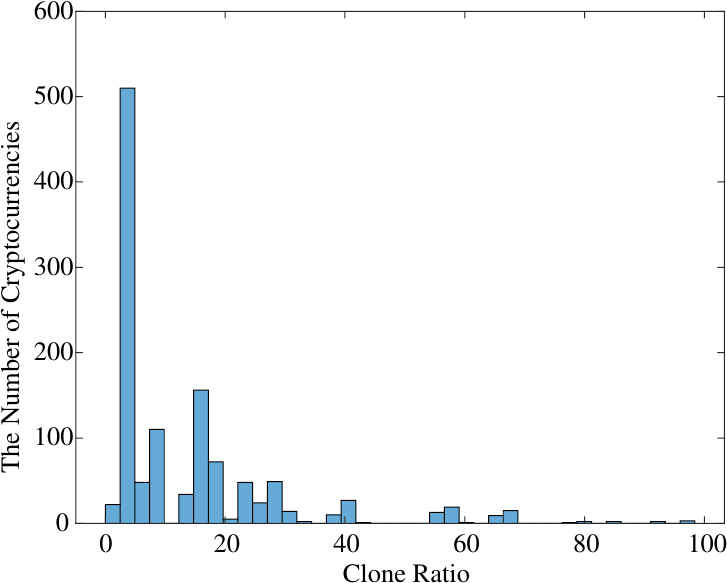
\includegraphics[width=0.5\textwidth]{obrazky-figures/clone_ratio_histogram.png}
      \caption{Bitcoin v0.17.0 clone ratio in forked projects. Source:~\cite{CoinWatch}}
      \label{bitcoin-clone-ratio}
    \end{figure}

    The overall workflow of CoinWatch is visualised in Figure \ref{coinwatch-workflow}. At the beginning
    of the pipeline, the tool receives a target CVE assigned to the target project. Accordingly, all publicly
    available details about the desired vulnerability are scraped and parsed from vulnerability databases.
    These details are input for the next step -- code evolution analysis. The analysis utilizes the version
    control system Git for traversing the versions of the target project. Using the parsed CVE details,
    the analysis aims to identify fixing and bug-introducing commits for the provided vulnerability
    in the project's repository. Identified fixing and bug-introducing commits form a time window, in which
    the target project was affected by the vulnerability. This time window is used for the initial filtering
    of potentially affected child projects, which were forked from the target project during this period.
    The identified fixing and bug-introducing commits are additionally used for manual annotation of
    the vulnerable code and transformation to a clone detection pattern. In the end, the clone detection tool
    checks the occurrence of the pattern in the potentially vulnerable projects forked in the time window.
    After clone detection, on the output of the pipeline is a list of likely affected cryptocurrencies.

    \begin{figure}[h]
      \centering
      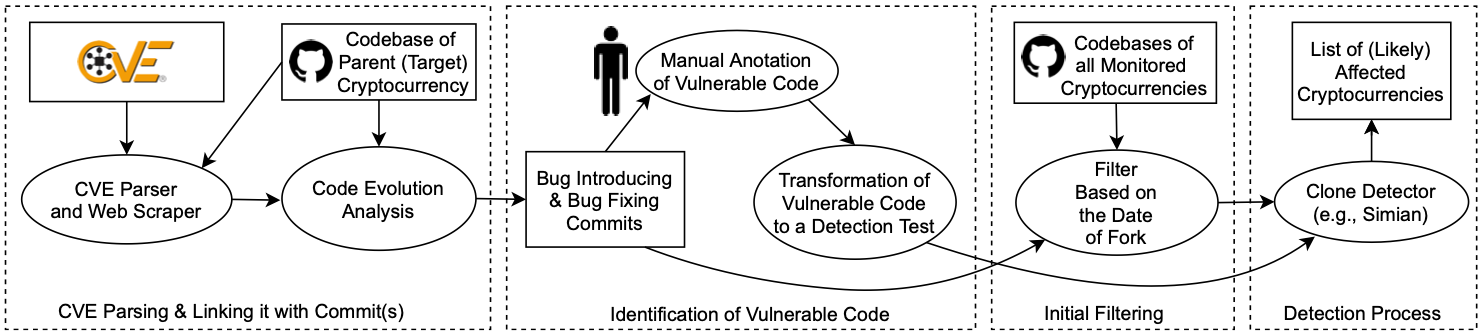
\includegraphics[width=1\textwidth]{obrazky-figures/coinwatch_workflow.png}
      \caption{Overall workflow of tool CoinWatch. Source:~\cite{CoinWatch}}
      \label{coinwatch-workflow}
    \end{figure}

    \subsubsection*{CVE Parsing and Linking with Commits}
      In this step, CoinWatch scrapes and parses details of the selected vulnerability. Following data
      are extracted from details about CVE in vulnerability databases:
      \begin{itemize}
          \item date of publishing
          \item keywords from description
          \item references pointing to the version control system of the affected project
          \item the list of affected cryptocurrencies and their programming language
      \end{itemize}
      After parsing, the origin of the vulnerability is checked, whether the issue is connected with specific
      code as the threat may originate from using outdated versions of libraries, frameworks and protocols.
      In case of code-specific weakness, the code evolution analysis links patching and bug-introducing
      commits with the CVE.

    \subsubsection*{Code Evolution Analysis -- SZZ Algorithm}
    For purpose of code evolution analysis, CoinWatch utilizes the SZZ algorithm. The algorithm was proposed
    by Sliwerski, Zimmermann and Zeller~\cite{SZZalgorithm} as an approach for identifying bug-introducing
    commits. An open implementation of the algorithm is named SZZ Unleashed~\cite{SZZunleashed}. It is written
    in Java programming language with supporting Python scripts. SZZ Unleashed works in two phases. The first
    phase identifies bug-fixing commits used in the second phase for tracking the bug-introducing changes.
    CoinWatch is built on this algorithm and extended it for the tool's specific purposes.

    Firstly, using parsed details about the vulnerability, the bug-fixing commits are identified from
    the version control system in the affected project. In CoinWatch this is done by matching regular expression
    in issues which have been fixed, resolved, closed or labelled as "bug". The regular expression is built
    from keywords extracted from the description in CVE details and keywords "CVE" and "CVE-ID".

    Secondly, for each discovered fixing commit the bug-introducing commits are tracked utilizing the second
    phase of the SZZ algorithm. This phase leverages the command git-blame and line number mapping to backtrack
    through the history of the analysed project. This method maps only the lines affected by the
    analysed commit as shown in Figure \ref{szz-line-map}. In addition, this phase provides an option to
    select the desired depth of mapping the line numbers over a variable number of versions, indicated by
    the depth parameter. In the provided example, working with the depth option set to one would result in
    not identifying the bug introduced by Commit 2, because it is in depth two and it is detectable only from
    the annotation of commits 3, 4 and 5.

    % note: Fix Commit Identification - https://www.st.cs.uni-saarland.de/papers/msr2005/msr2005.pdf
    \subsubsection*{Identification of Vulnerable Code and Initial Filtering}
    Inputs for this part of the CoinWatch are bug-fixing and their matching bug-introducing commits.
    For initial filtering of potentially vulnerable forks, CoinWatch selects the newest bug-fixing commit
    and the oldest bug-introducing commit to form a time window. Monitored forked projects are then filtered
    based on the timestamp of their fork. When it is within the time window they are marked as potentially
    vulnerable candidates. The projects around the time window are ignored.

    Identification of vulnerable code is a one-time manual process per CVE. The goal of this step is to
    extract the patch code and the vulnerable code from commits detected during code evolution analysis.
    After the manual code annotation, it is transformed into a detection test as input for the clone detection
    tool.

    \subsubsection*{Clone Detection Process}
    Finally, CoinWatch triggers the clone detection tool Simian \ref{clone-detection:simian} with the detection
    test on the list of potentially vulnerable candidates from the previous step. This filters the projects
    that already patched the vulnerability or reimplemented the part of code, which was vulnerable in the
    source project and returns the final list of likely vulnerable projects.

  \begin{figure}[h]
      \centering
      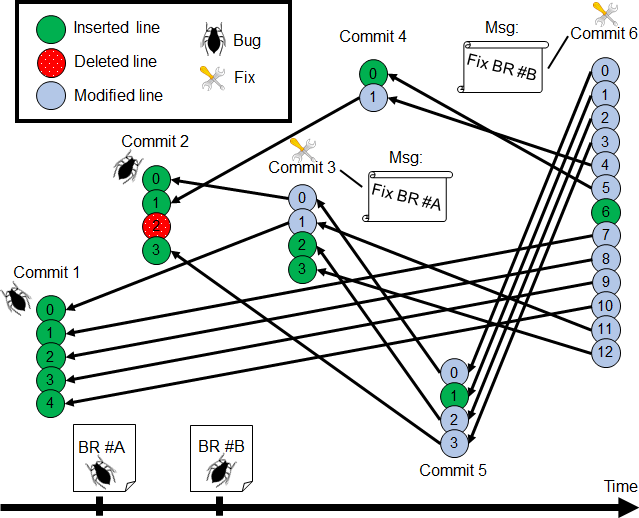
\includegraphics[width=0.7\textwidth]{obrazky-figures/szz_line_mapping.png}
      \caption{An example of SZZ Unleashed mapping line numbers. Source:~\cite{SZZunleashed}}
      \label{szz-line-map}
  \end{figure}

  \subsection*{BlackScope}
    BlockScope is a novel tool for detecting vulnerabilities propagated by cloning blockchain projects like
    Bitcoin and Ethereum. It is a language-agnostic tool capable of detecting multiple vulnerabilities from
    existing security patches. BlockScope utilizes similarity-based code match and designs
    a new way of calculating code similarity. Thanks to this approach it is able to detect Type~I, Type~II and
    Type~III clones. Additionally, it is capable of automatic extraction of security patch contexts in comparison
    to CoinWatch.

    Figure \ref{blockscopeworkflow} presents the overall workflow of BlockScope. In the beginning,
    the tool receives a security patch and the affected project on the input. The security patch is accepted
    either in form of a commit id from the source project or manually crafted patch contexts for better accuracy.
    A~patch context represents a surrounding of the code changes in the patch commit. The component named
    Extractor serves for identifying patch context when the commit id of a security patch is provided.
    Subsequently, the component Searcher tries to match the patch context in the analysed project which produces
    a candidate context. Then Fetcher uses the contexts for extraction of patch code from the source project
    and potentially vulnerable candidate code from the target project. The similarity of the extracted
    codes is then measured in Comparator, which determines whether the target project was patched. Additionally,
    for the vulnerabilities that were already fixed in the target repository, BlockScope performs
    the calculation of patch delay.

    \begin{figure}[h]
      \centering
      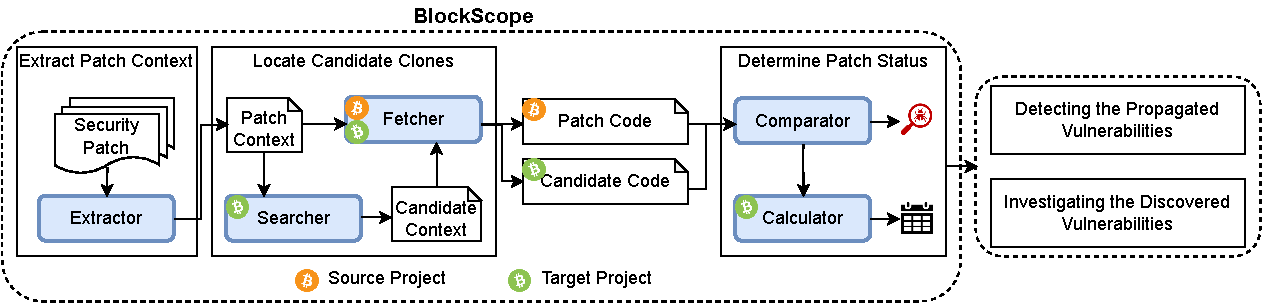
\includegraphics[width=0.99\textwidth]{obrazky-figures/blockscope_workflow.pdf}
      \caption{Overall workflow of tool BlockScope. Source:~\cite{BlockScope}}
      \label{blockscopeworkflow}
    \end{figure}

    BlockScope achieved overall precision and recall both at the rate of 91.8\%. It discovered 101 previously
    unknown vulnerabilities propagated via code cloning in 13 out of 16 analysed projects forked from Bitcoin
    and Ethereum. Unfortunately, just like CoinWatch it is not available for public use and is
    close sourced~\cite{BlockScope}.


% https://www.researchgate.net/publication/335152710_Detecting_Security_Vulnerabilities_using_Clone_Detection_and_Community_Knowledge

\chapter{Design}
\label{chapter:design}
  % idea: reverse SNMP system architecture
  % Central Database Server - data containing CVE mapping to source project, patch commit and patch code
  %   (possibly more details could be stored)
  % Tool as Agent - requests CVE details from the central server for the tool to operate: source project, patch commit
  %   and code


\chapter{Implementation}
\label{chapter:implementation}


\chapter{Experimentation}
\label{chapter:experimentation}


\chapter{Conclusion}
\label{chapter:conclusion}
